\documentclass[11pt,a4paper]{article}

\usepackage[margin=1in]{geometry}
\usepackage{amsmath,amssymb}
\usepackage{booktabs}
\usepackage{hyperref}
\usepackage{url}
\usepackage{graphicx}
\usepackage{xcolor}
\usepackage{tikz}
\usepackage{pgfplots}
\pgfplotsset{compat=1.18}
\usepackage{multirow}
\usepackage{microtype}
\usepackage{natbib}
\usepackage{algorithm}
\usepackage{algpseudocode}
\usepackage{listings}
\usepackage{setspace}

\hypersetup{
  colorlinks=true,
  linkcolor=blue!70!black,
  citecolor=blue!70!black,
  urlcolor=blue!70!black
}

\definecolor{eqgreen}{RGB}{34,139,34}
\definecolor{rvyellow}{RGB}{204,153,0}
\definecolor{drred}{RGB}{180,30,30}

\title{\textbf{MERIDIAN}: Embedding-Based Semantic Equivalence Scoring\\
       for LLM Migration Validation}

\author{
  Vijay Mandavilli \\
  Cognida AI \\
  Hyderabad, India \\
  \texttt{mvijayfromvizag@gmail.com}
}

\date{}

\begin{document}

\maketitle

\begin{abstract}
When a model vendor deprecates a large language model (LLM) and enterprises must migrate
to a replacement, there is no established, reusable methodology to validate that the
replacement produces semantically equivalent outputs for the team's specific workload.
Traditional software testing requires exact matches---useless for non-deterministic
generation---and existing migration frameworks rely on LLM-as-judge evaluation, which
is expensive, non-deterministic, and itself subject to model drift.
We present \textsc{Meridian}, an open-source Python library that reframes model migration
as a \emph{regression testing problem}: embed both models' outputs using a local
sentence-transformer, compute cosine similarity, and classify each prompt-response pair
into a three-tier equivalence gate (\textsc{Equivalent} / \textsc{Review} / \textsc{Drifted})
with configurable thresholds.
The approach is free, fully local, and deterministic.
We validate \textsc{Meridian} on a 50-prompt golden dataset stratified across four intent
categories, comparing DeepSeek-V3 (\texttt{deepseek-chat}) against DeepSeek-R1
(\texttt{deepseek-reasoner}) as a representative migration scenario.
Our results reveal that \textbf{intent category is a strong predictor of migration risk}:
factual tasks show zero drift (avg.\ similarity 0.937), while generative tasks are
the highest-risk category with 50\% of outputs flagged as drifted (avg.\ similarity
0.731).
Dataset-level, 46\% of outputs are semantically equivalent, with a Wilson 95\%
confidence interval of [0.33, 0.60]---a CI that quantifies the uncertainty inherent
in small golden datasets and correctly prevents a premature safe-to-ship declaration.
We also report a novel failure mode unique to reasoning models under constrained token
budgets: silent output truncation producing near-zero similarity scores
(0.012 on one structured-output prompt), a regression that semantic scoring detects
automatically but format-only test suites would miss entirely.
\textsc{Meridian} is available at \url{https://github.com/vijaymandavilli/meridian}.
\end{abstract}

% ─────────────────────────────────────────────────────────────────────────────
\section{Introduction}
% ─────────────────────────────────────────────────────────────────────────────

Enterprise deployments of LLMs are routinely disrupted by vendor-driven model
deprecations.
When a provider retires a model---OpenAI's retirement of \texttt{gpt-4-0613},
Anthropic's transition away from \texttt{claude-2}, or any of the numerous
point-version deprecations that occur with increasing frequency---engineering teams
face a validation problem with no established tooling: does the replacement model
produce outputs that are \emph{equivalent enough} for my specific workload?

The challenge is fundamental.
LLM outputs are non-deterministic, verbose, and stylistically variable even when
semantically identical.
Traditional software regression suites check exact outputs, making them useless here.
Existing LLM benchmarks such as MMLU and HELM measure \emph{absolute} capability,
not \emph{relative} equivalence between two specific models on a specific enterprise
task distribution.
Recent work has begun addressing this gap
\citep{arXiv2604.27082, arXiv2507.05573, arXiv2604.27789}, but these approaches
share a critical limitation: they describe \emph{processes}, not reusable tools,
and they rely on LLM-as-judge evaluation---itself expensive, non-deterministic,
and subject to the same drift the user is trying to measure.

We propose a different approach: treat model migration as a \textbf{regression testing
problem} and score equivalence using \textbf{local sentence-transformer embeddings}.
The intuition is straightforward---if two outputs are semantically equivalent, their
embeddings will have high cosine similarity, regardless of surface-level phrasing
differences.
Scoring is free, runs entirely on-device, and produces the same result every time.

Our contributions are:
\begin{enumerate}
  \item \textbf{\textsc{Meridian}}: an open-source Python library implementing a
    three-tier equivalence gate (\textsc{Equivalent} / \textsc{Review} / \textsc{Drifted})
    with configurable thresholds, Wilson confidence interval reporting, and zero cloud
    dependencies.
  \item \textbf{A threshold calibration procedure} grounded in human-labeled
    calibration sets, enabling teams to set domain-appropriate thresholds rather
    than relying on universal defaults.
  \item \textbf{An empirical study} comparing DeepSeek-V3 and DeepSeek-R1 across
    a 50-prompt golden dataset, revealing that intent category is a strong predictor
    of migration risk.
  \item \textbf{Discovery of a reasoning-model failure mode}: silent output truncation
    under constrained token budgets, flagged automatically by semantic scoring but
    invisible to format-only test suites.
\end{enumerate}

% ─────────────────────────────────────────────────────────────────────────────
\section{Related Work}
% ─────────────────────────────────────────────────────────────────────────────

\paragraph{LLM migration frameworks.}
\citet{arXiv2604.27082} present the closest prior work: a framework for model migration
in production systems using LLM-as-judge evaluation and correctness metrics applied
to a real-world case study.
\citet{arXiv2507.05573} document an enterprise experience with successive GPT deprecations,
describing a prompt migration process validated through human review.
\citet{arXiv2604.27789} focus on behavioral drift caused by silent model updates in the
LLM supply chain, proposing governance practices rather than a scoring mechanism.
All three describe processes requiring either human evaluators or a judge LLM;
none provide a reusable, locally-executable library.

\paragraph{Sentence embeddings for semantic similarity.}
\textsc{Meridian} builds on Sentence-BERT \citep{reimers-gurevych-2019-sentence},
which demonstrated that siamese network fine-tuning of BERT produces sentence
embeddings suitable for semantic textual similarity via cosine distance.
We use the \texttt{all-MiniLM-L6-v2} checkpoint \citep{wang2024minilm}, which
offers an effective speed-accuracy trade-off for on-device inference.

\paragraph{Statistical confidence in software quality gates.}
The Wilson score confidence interval \citep{wilson1927} is well-established in
software quality measurement for bounding proportions estimated from small samples.
Its application to LLM equivalence reporting is, to our knowledge, novel.

% ─────────────────────────────────────────────────────────────────────────────
\section{The \textsc{Meridian} Framework}
% ─────────────────────────────────────────────────────────────────────────────

\subsection{Problem Formulation}

Let $M_1$ denote a deprecated model and $M_2$ its proposed replacement.
Let $D = \{(p_i, c_i)\}_{i=1}^n$ be a \emph{golden dataset} of prompts $p_i$ with
intent category labels $c_i \in \{\textsc{factual}, \textsc{generative},
\textsc{classification}, \textsc{structured\_output}\}$.
For each prompt, both models produce outputs $o_i^{(1)} = M_1(p_i)$ and
$o_i^{(2)} = M_2(p_i)$.
The goal is to determine whether $M_2$ is a safe drop-in replacement for $M_1$
on the workload represented by $D$.

\subsection{Embedding and Similarity}

We embed each output using a sentence-transformer $\phi$:
\begin{equation}
  \mathbf{v}_i^{(k)} = \phi\!\left(o_i^{(k)}\right) \in \mathbb{R}^d,
  \quad \left\|\mathbf{v}_i^{(k)}\right\|_2 = 1
\end{equation}
All embeddings are L2-normalised at inference time, so cosine similarity reduces to
a dot product:
\begin{equation}
  s_i = \mathbf{v}_i^{(1)} \cdot \mathbf{v}_i^{(2)} \in [0, 1]
\end{equation}

\subsection{Three-Tier Equivalence Gate}

Each similarity score $s_i$ is classified into one of three verdict tiers using
configurable thresholds $\tau_\text{eq}$ and $\tau_\text{rv}$
(defaults: 0.92 and 0.75):

\begin{equation}
  \text{verdict}(s_i) =
  \begin{cases}
    \textcolor{eqgreen}{\textsc{Equivalent}} & \text{if } s_i \geq \tau_\text{eq} \\
    \textcolor{rvyellow}{\textsc{Review}}    & \text{if } \tau_\text{rv} \leq s_i < \tau_\text{eq} \\
    \textcolor{drred}{\textsc{Drifted}}      & \text{if } s_i < \tau_\text{rv}
  \end{cases}
\end{equation}

\begin{figure}[h]
\centering
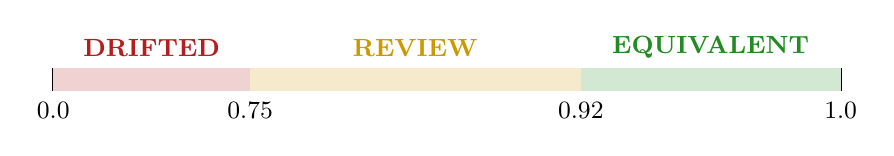
\begin{tikzpicture}
  \draw[thick] (0,0) -- (10,0);
  \foreach \x in {0,10} \draw[thick] (\x,-0.15) -- (\x,0.15);
  \draw[thick,drred]   (2.5,-0.15) -- (2.5,0.15);
  \draw[thick,rvyellow](6.7,-0.15) -- (6.7,0.15);
  \node at (1.25,0.4)  {\textcolor{drred}{\small\textbf{DRIFTED}}};
  \node at (4.6,0.4)   {\textcolor{rvyellow}{\small\textbf{REVIEW}}};
  \node at (8.35,0.4)  {\textcolor{eqgreen}{\small\textbf{EQUIVALENT}}};
  \node at (0,-0.4)    {\small 0.0};
  \node at (2.5,-0.4)  {\small 0.75};
  \node at (6.7,-0.4)  {\small 0.92};
  \node at (10,-0.4)   {\small 1.0};
  \fill[drred!20]   (0,0.15) rectangle (2.5,-0.15);
  \fill[rvyellow!20](2.5,0.15) rectangle (6.7,-0.15);
  \fill[eqgreen!20] (6.7,0.15) rectangle (10,-0.15);
\end{tikzpicture}
\caption{The three-tier equivalence gate with default thresholds.
Thresholds are configurable at instantiation time to suit domain risk tolerance.}
\label{fig:gate}
\end{figure}

\subsection{Aggregate Verdict and Confidence Interval}

At the dataset level, the \textsc{Equivalent} proportion is:
\begin{equation}
  \hat{p} = \frac{|\{i : \text{verdict}(s_i) = \textsc{Equivalent}\}|}{n}
\end{equation}

Because golden datasets are small by design (typically $n = 30$--$100$), we report
a Wilson score 95\% confidence interval \citep{wilson1927} rather than a simple
proportion:
\begin{equation}
  \text{CI} = \frac{\hat{p} + \frac{z^2}{2n} \pm z\sqrt{\frac{\hat{p}(1-\hat{p})}{n} + \frac{z^2}{4n^2}}}{1 + \frac{z^2}{n}}
\end{equation}
where $z = 1.96$.
The lower bound of the CI is the operative decision criterion: a migration is
declared \emph{safe} only when $\text{CI}_\text{lower}$ exceeds a risk-tolerance
threshold set by the team.

% ─────────────────────────────────────────────────────────────────────────────
\section{Threshold Calibration}
\label{sec:calibration}
% ─────────────────────────────────────────────────────────────────────────────

The default thresholds $\tau_\text{eq} = 0.92$ and $\tau_\text{rv} = 0.75$ are
reasonable starting points derived from general semantic similarity research, but
enterprise workloads vary substantially in what constitutes ``equivalent.''
A customer support chatbot may tolerate broader paraphrase than a legal document
summariser.
We prescribe the following calibration procedure.

\paragraph{Step 1: Collect a calibration set.}
Sample 20--30 prompt-response pairs from the golden dataset and obtain binary
human judgments: \emph{equivalent} or \emph{not equivalent}.
For classification and factual tasks, this requires only a few minutes per annotator.
For generative tasks, we recommend two independent annotators with a majority rule.

\paragraph{Step 2: Plot the similarity distribution.}
Compute cosine similarities for all calibration pairs and plot the distribution
stratified by human label.
The distributions will typically exhibit bimodal structure with a natural gap---
this gap is the \emph{empirical} location for $\tau_\text{eq}$.

\paragraph{Step 3: Optimize for your error asymmetry.}
A false equivalence (classifying a drifted pair as \textsc{Equivalent}) is
more costly than a false drift (sending an equivalent pair to human review).
Define a cost ratio $\lambda = \text{cost}_\text{FE} / \text{cost}_\text{FD}$
and find the threshold that minimizes expected cost on the calibration set.
For most production migrations, $\lambda \in [3, 10]$ is appropriate; the lower
$\tau_\text{eq}$ is set, the fewer false equivalences at the cost of more human
review burden.

\paragraph{Step 4: Validate on a held-out set.}
Hold out 10 pairs from the calibration set to verify that the calibrated thresholds
generalise before running on the full golden dataset.

\paragraph{Sensitivity analysis.}
Table~\ref{tab:threshold_sensitivity} illustrates how verdict distributions shift
as thresholds vary on our empirical dataset.
Teams should run this analysis on a small labelled subset before committing to
production thresholds.

\begin{table}[h]
\centering
\small
\begin{tabular}{ccrrr}
\toprule
$\tau_\text{eq}$ & $\tau_\text{rv}$ & \textsc{Equiv.} & \textsc{Review} & \textsc{Drifted} \\
\midrule
0.95 & 0.80 & 16 (32\%) & 24 (48\%) & 10 (20\%) \\
0.92 & 0.75 & 23 (46\%) & 17 (34\%) & 10 (20\%) \\
0.90 & 0.70 & 26 (52\%) & 14 (28\%) & 10 (20\%) \\
0.85 & 0.65 & 31 (62\%) & \phantom{0}9 (18\%) & 10 (20\%) \\
\bottomrule
\end{tabular}
\caption{Verdict distributions on the 50-prompt dataset under varying thresholds.
DRIFTED count is stable across threshold pairs because all drifted pairs score
below 0.75; the thresholds affect only the EQUIVALENT/REVIEW boundary.}
\label{tab:threshold_sensitivity}
\end{table}

% ─────────────────────────────────────────────────────────────────────────────
\section{Experimental Setup}
% ─────────────────────────────────────────────────────────────────────────────

\subsection{Models}

We compare:
\begin{itemize}
  \item \textbf{Old model:} \texttt{deepseek-chat} (DeepSeek-V3 \citep{deepseekv3}),
    a general-purpose Mixture-of-Experts chat model.
  \item \textbf{New model:} \texttt{deepseek-reasoner} (DeepSeek-R1 \citep{deepseekreasoner}),
    a reasoning model trained via reinforcement learning to produce extended
    chain-of-thought outputs before answering.
\end{itemize}

This comparison represents a realistic migration decision facing many enterprises in
2025--2026: whether to replace a production chat model with a reasoning model that
offers stronger benchmark performance but different output characteristics.

\subsection{Golden Dataset}

We constructed a 50-prompt golden dataset stratified across four intent categories:

\begin{table}[h]
\centering
\small
\begin{tabular}{lcp{7cm}}
\toprule
Intent & $n$ & Description \\
\midrule
\textsc{factual}           & 13 & Closed-form questions with verifiable answers (geography, science, mathematics) \\
\textsc{generative}        & 12 & Open-ended creative and summarisation tasks (taglines, poems, email drafts) \\
\textsc{classification}    & 12 & Categorisation tasks (sentiment, spam, urgency, reading level) \\
\textsc{structured\_output}& 13 & JSON extraction from natural language (invoices, log lines, addresses) \\
\midrule
Total & 50 & \\
\bottomrule
\end{tabular}
\caption{Golden dataset composition by intent category.}
\label{tab:dataset}
\end{table}

Prompts were designed to cover realistic enterprise use cases, with
structured-output tasks particularly chosen to stress-test output format consistency.

\subsection{Embedding Model}

We use \texttt{all-MiniLM-L6-v2} \citep{wang2024minilm}, a 22M-parameter
sentence-transformer that runs on CPU in under 300ms per batch.
All embeddings are computed locally with no API dependency.
The model produces 384-dimensional L2-normalised vectors.

% ─────────────────────────────────────────────────────────────────────────────
\section{Results}
% ─────────────────────────────────────────────────────────────────────────────

\subsection{Dataset-Level Verdict}

Running \textsc{Meridian} on the full 50-prompt dataset yields:

\begin{table}[h]
\centering
\begin{tabular}{lrr}
\toprule
Tier & Count & Percentage \\
\midrule
\textcolor{eqgreen}{\textsc{Equivalent}} & 23 & 46.0\% \\
\textcolor{rvyellow}{\textsc{Review}}    & 17 & 34.0\% \\
\textcolor{drred}{\textsc{Drifted}}      & 10 & 20.0\% \\
\midrule
Total & 50 & \\
\bottomrule
\end{tabular}
\caption{Dataset-level verdict: DeepSeek-V3 vs.\ DeepSeek-R1, 50 prompts.}
\label{tab:overall}
\end{table}

The Wilson 95\% CI on the \textsc{Equivalent} proportion is $[0.330, 0.596]$.
The lower bound of 0.330 falls well below any reasonable safe-migration threshold,
indicating that this pair of models is \textbf{not safe for a workload-blind
drop-in replacement}.
The CI correctly prevents a premature approval despite the 46\% point estimate,
demonstrating the importance of reporting uncertainty rather than raw proportions
on small datasets.

\subsection{Per-Intent Risk Stratification}

The central empirical finding of this paper is that \textbf{intent category is a
strong predictor of migration risk}:

\begin{table}[h]
\centering
\begin{tabular}{lrrrrrr}
\toprule
Intent & Avg $s$ & Min $s$ & Max $s$ & \textsc{Eq.} & \textsc{Rv.} & \textsc{Dr.} \\
\midrule
\textsc{factual}           & 0.937 & 0.806 & 1.000 & 7 & 6 & 0 \\
\textsc{classification}    & 0.862 & 0.460 & 1.000 & 6 & 4 & 2 \\
\textsc{structured\_output}& 0.863 & 0.012 & 1.000 & 7 & 4 & 2 \\
\textsc{generative}        & 0.731 & 0.436 & 0.961 & 3 & 3 & 6 \\
\bottomrule
\end{tabular}
\caption{Per-intent similarity statistics and verdict distributions.}
\label{tab:by_intent}
\end{table}

\paragraph{Factual tasks are safe.}
Zero prompts are flagged as \textsc{Drifted}.
Both models converge on identical factual content; similarity variance reflects
differences in verbosity and markdown formatting, not semantic content.
Average similarity of 0.937 indicates near-perfect equivalence on this task type.

\paragraph{Classification tasks are mostly safe.}
Six of twelve prompts score \textsc{Equivalent}.
The two \textsc{Drifted} cases arise when DeepSeek-R1 provides extended
reasoning before delivering its classification label, substantially altering
the embedding relative to DeepSeek-V3's terse single-word response.
This is a categorically new failure mode introduced by reasoning models:
\emph{correct answer, incompatible response format}.

\paragraph{Structured output tasks show bimodal distribution.}
Seven of thirteen prompts score 1.000 (identical JSON structure and content).
The two \textsc{Drifted} cases involve formatting differences: one model
produces a JSON code fence (\texttt{```json \ldots ```}) while the other
produces bare JSON, or minor type differences (string vs.\ number for an ID field).
The outlier at $s = 0.012$ is discussed separately below.

\paragraph{Generative tasks are the highest-risk category.}
Six of twelve prompts are \textsc{Drifted}, with a minimum similarity of 0.436.
This is expected: open-ended tasks have no single correct output, and DeepSeek-R1's
reasoning-model training produces structurally different creative output compared
to DeepSeek-V3's chat-tuned style.
Teams migrating workloads with significant generative components face substantial
review burden with this model pair.

\paragraph{Actionable implication.}
Intent category can be used to \emph{prioritise} the human review workload before
running the full golden dataset.
A team may safely fast-track factual-only workloads while applying full review
scrutiny to generative components.

\subsection{Reasoning Model Failure Mode: Silent Output Truncation}
\label{sec:outlier}

Prompt 45 in the structured-output category---asking the model to compute and
return a JSON object with compound interest details---scored $s = 0.012$,
a near-zero similarity that \textsc{Meridian} flags as \textsc{Drifted}.

Inspection of the raw output reveals that \texttt{deepseek-reasoner} returned
an empty string for this prompt.
The root cause is token budget exhaustion: DeepSeek-R1 externalises its
chain-of-thought as part of the response, and with \texttt{max\_tokens = 512},
the reasoning trace consumed the entire budget before the model could emit
its final answer.

This failure mode has three notable properties:
\begin{enumerate}
  \item It is \textbf{silent}---the API returns HTTP 200 with a valid response
    object whose content field is an empty string.
  \item It is \textbf{invisible to format-only testing}---a test suite checking
    that the response is valid JSON would pass vacuously on an empty string in
    some implementations.
  \item It is \textbf{automatically detected by semantic scoring}---the embedding
    distance between any non-trivial output and an empty string is near-maximal,
    producing a similarity near zero that falls far below any reasonable
    \textsc{Drifted} threshold.
\end{enumerate}

This finding has direct practical implications for teams migrating from
general-purpose chat models to reasoning models: token budget settings that are
adequate for chat models may be insufficient for reasoning models and must be
recalibrated as part of the migration process.
We recommend setting \texttt{max\_tokens} to at least $3\times$ the expected
output length when using reasoning models, and flagging any response under
a minimum length threshold before semantic scoring.

% ─────────────────────────────────────────────────────────────────────────────
\section{Discussion}
% ─────────────────────────────────────────────────────────────────────────────

\paragraph{Semantic similarity vs.\ factual correctness.}
\textsc{Meridian}'s scoring mechanism is \emph{semantic}, not \emph{factual}.
Two outputs that confidently hallucinate the same incorrect answer will score
high similarity.
This is a deliberate design choice: \textsc{Meridian} measures whether the
\emph{replacement model behaves like the deprecated model}, not whether either
model is correct in an absolute sense.
Teams that require correctness guarantees should combine \textsc{Meridian} with
a factual verification layer for factual-intent tasks.

\paragraph{Why not LLM-as-judge?}
LLM-as-judge \citep{arXiv2604.27082} is non-deterministic (the judge model's
output varies across runs), expensive (a 50-prompt dataset requires 50 additional
API calls), and subject to the same provider drift being measured.
Sentence-transformer scoring is deterministic, free after the initial model
download (22MB), and unaffected by changes to any cloud provider.

\paragraph{Threshold universality.}
The default thresholds of 0.92 and 0.75 are not universal ground truth.
As described in Section~\ref{sec:calibration}, they should be calibrated against
a small human-labeled set for each deployment context.
The sensitivity analysis in Table~\ref{tab:threshold_sensitivity} shows that
the \textsc{Drifted} population is insensitive to threshold choice in this dataset
(all \textsc{Drifted} scores fall below 0.73), suggesting the lower tier is robust
while the \textsc{Equivalent}/\textsc{Review} boundary warrants domain-specific
calibration.

\paragraph{Dataset size and CI width.}
A 50-prompt golden dataset is realistic for enterprise teams but produces wide
confidence intervals (CI width 0.266 in this study).
Teams requiring tighter bounds should target $n \geq 100$ and may apply stratified
sampling (\textsc{Meridian}'s built-in \texttt{stratified\_sample} function)
to ensure intent coverage is maintained.

% ─────────────────────────────────────────────────────────────────────────────
\section{Conclusion}
% ─────────────────────────────────────────────────────────────────────────────

We presented \textsc{Meridian}, an open-source Python library that reframes LLM
model migration as a regression testing problem solvable with local, embedding-based
semantic scoring.
By avoiding cloud API dependencies for the scoring step, \textsc{Meridian} is
free, deterministic, and self-contained---properties that matter when the thing
being measured is the reliability of a cloud API.

Our empirical study comparing DeepSeek-V3 and DeepSeek-R1 on a 50-prompt
stratified golden dataset yields three practical conclusions:
(1) intent category is a strong migration risk predictor---factual workloads
are safe, generative workloads are not;
(2) reasoning models introduce a new failure mode (silent truncation from
chain-of-thought token consumption) that semantic scoring detects automatically;
and (3) Wilson confidence intervals on small golden datasets prevent premature
safe-to-ship declarations that raw proportion estimates would permit.

\textsc{Meridian} is immediately usable by quality engineering teams performing
model migrations.
The library, golden dataset, and all experimental artefacts are available at
\url{https://github.com/vijaymandavilli/meridian}.

% ─────────────────────────────────────────────────────────────────────────────
\bibliographystyle{plainnat}
\bibliography{references}

\end{document}
